\documentclass[11pt,a4paper]{article}
\usepackage[T1]{fontenc}
\usepackage[utf8]{inputenc}
\usepackage{lmodern,microtype,graphicx,booktabs,tabularx,array,amsmath,amssymb}
\usepackage[margin=22mm]{geometry}
\usepackage[colorlinks=true,linkcolor=black,citecolor=black,urlcolor=blue]{hyperref}
\usepackage[numbers,sort&compress]{natbib}
\usepackage{caption,float}
\usepackage[section]{placeins}
\captionsetup{font=small,labelfont=bf}
\renewcommand{\topfraction}{0.95}
\renewcommand{\bottomfraction}{0.9}
\renewcommand{\textfraction}{0.05}
\renewcommand{\floatpagefraction}{0.8}
\widowpenalty=10000
\clubpenalty=10000
\setlength{\parskip}{4pt}
\setlength{\parindent}{12pt}
\setlength{\emergencystretch}{1.5em}
\newcommand{\co}{CO\textsubscript{2}}
\newcommand{\rr}{CO\textsubscript{2}RR}
\newcommand{\ca}{Cu--Au}
\title{An agentic framework for X-ray absorption spectroscopy of catalytic interfaces}
\author{\small Haili Jia\textsuperscript{1}, Pooja Basera\textsuperscript{2}, Dimosthenis Sokaras\textsuperscript{2},\\
\small Maria K. Y. Chan\textsuperscript{1,*}\\[0.6em]
\small \textsuperscript{1}Center for Nanoscale Materials, Argonne National Laboratory,\\
\small 9700 South Cass Avenue, Lemont, Illinois 60439, United States\\
\small \textsuperscript{2}SLAC National Accelerator Laboratory,\\
\small Menlo Park, California 94025, United States\\
\small \textsuperscript{*}Corresponding author: \href{mailto:mchan@anl.gov}{mchan@anl.gov}}
\hypersetup{pdftitle={An agentic framework for X-ray absorption spectroscopy of catalytic interfaces},pdfauthor={Haili Jia, Pooja Basera, Dimosthenis Sokaras, Maria K. Y. Chan}}
\date{}
\begin{document}
\maketitle
\begin{abstract}
Designing selective catalysts requires understanding how local atomic environments stabilize intermediates and redirect competing reaction pathways. X-ray absorption spectroscopy (XAS), including in situ and operando measurements, can follow changes in a working catalyst, but its ensemble-averaged response rarely identifies a transient interfacial state without suitable structural references. Here we present an agentic framework that connects controlled atomistic hypotheses to simulated spectra and predictive analysis. The workflow translates a catalytic question into interface construction, first-principles relaxation, supercomputer-based XAS calculations, AI-ready records, and machine-learning analysis. We demonstrate the framework for electrochemical CO\textsubscript{2} reduction (CO\textsubscript{2}RR), varying adsorbate identity, binding geometry, coverage, and distance from a Cu--Au interface. Models trained and evaluated through the agent recover adsorbate information from population-weighted Cu K-edge spectra, while depth-resolved comparisons quantify the loss of surface sensitivity. Clean-surface references define a signed differential response on a shared relative intensity scale, providing an input convention compatible with normalized experimental difference spectra. Absolute absorption per Cu atom is not required for identity inference. Expanded Cu--Au and Cu(100) analyses distinguish recoverable adsorbate and loading information from limitations associated with mixtures, sparse chemical environments and substrate dependence. Controlled enlargement of the training set gives a modest, statistically inconclusive improvement, indicating that chemical diversity and validation design remain as important as dataset size. By retaining the connection between a catalytic question, the relaxed chemical state, and its spectral response, the framework supports interpretable comparisons and selection of informative subsequent calculations.
\end{abstract}

\section{Introduction}
Improving catalytic selectivity requires identifying the atomic environments and intermediates that direct a reaction toward a desired product. Electrochemical CO\textsubscript{2} reduction (CO\textsubscript{2}RR) makes this challenge particularly acute: formation of ethylene or ethanol requires an overall transfer of 12 electrons per product molecule, while formation of n-propanol requires 18.\cite{ni2024,francis2018} These transfers occur through a network of adsorption, protonation, and bond-forming events whose branching depends on the catalyst and reaction environment. Distinguishing adsorbed CO from its hydrogenated or C--C-coupled derivatives is therefore central to evaluating proposed pathways.\cite{zhan2024,montoya2015}

The relevant catalyst structure must be established during operation. Applied potential, adsorbate coverage, and contact with the electrolyte can change the metal surface and its chemical state. Characterization performed only before or after reaction can miss these transformations. In situ measurements probe a catalyst within a controlled reaction environment; operando measurements additionally relate its state to simultaneously measured catalytic performance.\cite{operando2021} Time-resolved XAS during CO\textsubscript{2}RR, for example, has connected evolving Cu chemical states with product formation.\cite{lin2020}

XAS is especially useful because its element specificity and sensitivity to local coordination and electronic structure do not require long-range crystallinity. Hard X-rays can access catalysts inside electrochemical cells, allowing changes in oxidation state and metal environments to be followed during reaction.\cite{operando2021,lin2020} The interpretation remains challenging because the measured signal combines inequivalent absorbers: a small population near an adsorbate or interface may be obscured by the much larger metal background. A pathway hypothesis therefore requires more than assigning an oxidation state; it requires establishing whether the proposed intermediate and its local environment have a distinguishable spectral response.

Bimetallic interfaces offer useful catalytic functions while increasing the number of plausible local environments. Au--Cu tandem catalysts combine CO formation on Au with further reduction on Cu.\cite{morales2018} The resulting CO population and its proximity to Cu sites motivate a specific question: can XAS distinguish two neighboring CO molecules from a bonded OCCO intermediate, and does that contrast change near Au? The answer depends on local metal coordination, distance from the interface, molecular orientation, and spectator species. These variables must be controlled before a spectral difference can be attributed to a particular chemical step.

Reliable experimental spectrum--structure pairs can support this analysis, but independently labeling every transient adsorbate and interfacial geometry is difficult. Simulations provide an alternative source of labeled data and enable comparisons in which composition, coverage, or location is deliberately held fixed. Available approaches include real-space multiple scattering in FEFF, Green-function or finite-difference calculations in FDMNES, supercell core-excitation methods in VASP, and electron--hole treatments in OCEAN.\cite{rehr2010,joly2001,vasp1996,vaspxas,ocean2011} Choices of absorber ensemble, core-hole treatment, spatial extent, convergence, and processing affect the predicted spectral response. Incorrect adsorption geometry, propagation of an unrelaxed structure, or loss of chemical identity during calculation can consequently change the inferred chemistry, even when a calculation terminates successfully. The problem is both computational scale and scientific consistency.

These labeled spectra also make the inverse problem accessible to machine learning. Neural networks have reconstructed structural distributions from EXAFS and inferred local descriptors of bimetallic catalysts from XANES.\cite{timoshenko2018,marcella2020} Random forests have related near-edge spectra to coordination, mean nearest-neighbor distance, and Bader charge,\cite{torrisi2020} while convolutional neural networks have extracted bond-length information from molecular XAS.\cite{david2023} The appropriate model and target therefore depend on the physical question and the structural diversity represented in training. Featurization controls which spectral variations are retained and can improve robustness to differences between calculated and measured spectra.\cite{chen2024} Multimodal learning further combines complementary edges to infer local composition and defects that may be ambiguous in a single channel.\cite{jia2026}

For catalytic interfaces, realizing these capabilities requires a consistent link between the structural alternatives, their spectra, and the targets learned by the model. A classifier cannot distinguish competing intermediates if relaxation has changed their connectivity without updating the labels; nor can validation establish transfer if related spectra from one geometry appear in both training and testing. The computational workflow must therefore preserve chemical identity and sample independence as carefully as it manages numerical calculations. This requirement links structure generation, simulation, and inference into one scientific task.

Advances in language-model reasoning and tool use make it possible to coordinate this task through a scientific request, reducing repeated manual setup and the need to navigate each software interface separately. Chemistry agents can translate scientific requests into specialized computational actions,\cite{bran2024} while work on automated research platforms emphasizes the need to connect planning, execution, and interpretation through explicit interfaces.\cite{canty2023} Related agentic systems have automated structure preparation, high-performance-computing execution, and analysis for atomistic simulations.\cite{vriza2026} XAS adds the need to connect each chemical state to a specified absorbing-site ensemble and spectral representation. Here the objective is an end-to-end spectroscopy workflow in which the catalytic question remains connected to the structures, supercomputer calculations, and subsequent analysis. Chemical validation and numerical checks are essential because efficient execution alone cannot establish a chemically meaningful result.

We present an end-to-end framework for XAS of catalytic interfaces and demonstrate it with Cu--Au models relevant to CO\textsubscript{2}RR. The calculation agent connects natural-language requests to interface construction, first-principles relaxation and XAS at NERSC, while linked structural and spectral records support automated model training and evaluation. The resulting library allows adsorbate identity to be examined alongside coverage, local coordination and depth averaging. We further evaluate adsorption-induced differences against a separately calculated clean interface, following the physical motivation of adsorbate-sensitive difference XANES.\cite{ramaker2010,ramaker2014} Comparisons of raw and differential spectra on identical configurations assess the information retained by each representation, with source weighting and normalization treated as explicit controls. CO-loading and Cu(100) analyses then test how the inference depends on chemical composition and substrate-specific training data.

\section{An agentic workflow for interface spectroscopy}
\subsection{From catalytic hypotheses to computational comparisons}
The workflow begins with alternatives that a spectrum should distinguish, rather than with a fixed catalogue of calculations (Fig.~\ref{fig:framework}). For CO coupling at Cu--Au, the alternatives are neighboring CO molecules and a C--C-bonded intermediate. A useful comparison must hold elemental loading and the parent surface fixed while changing connectivity or interface location. The agent translates this intent into structured construction and calculation tasks. Dedicated scientific tools enforce the requested composition, adsorption region, and numerical settings, allowing the scientific question to remain explicit as it moves between different simulation codes.

\begin{figure}[!htbp]
\centering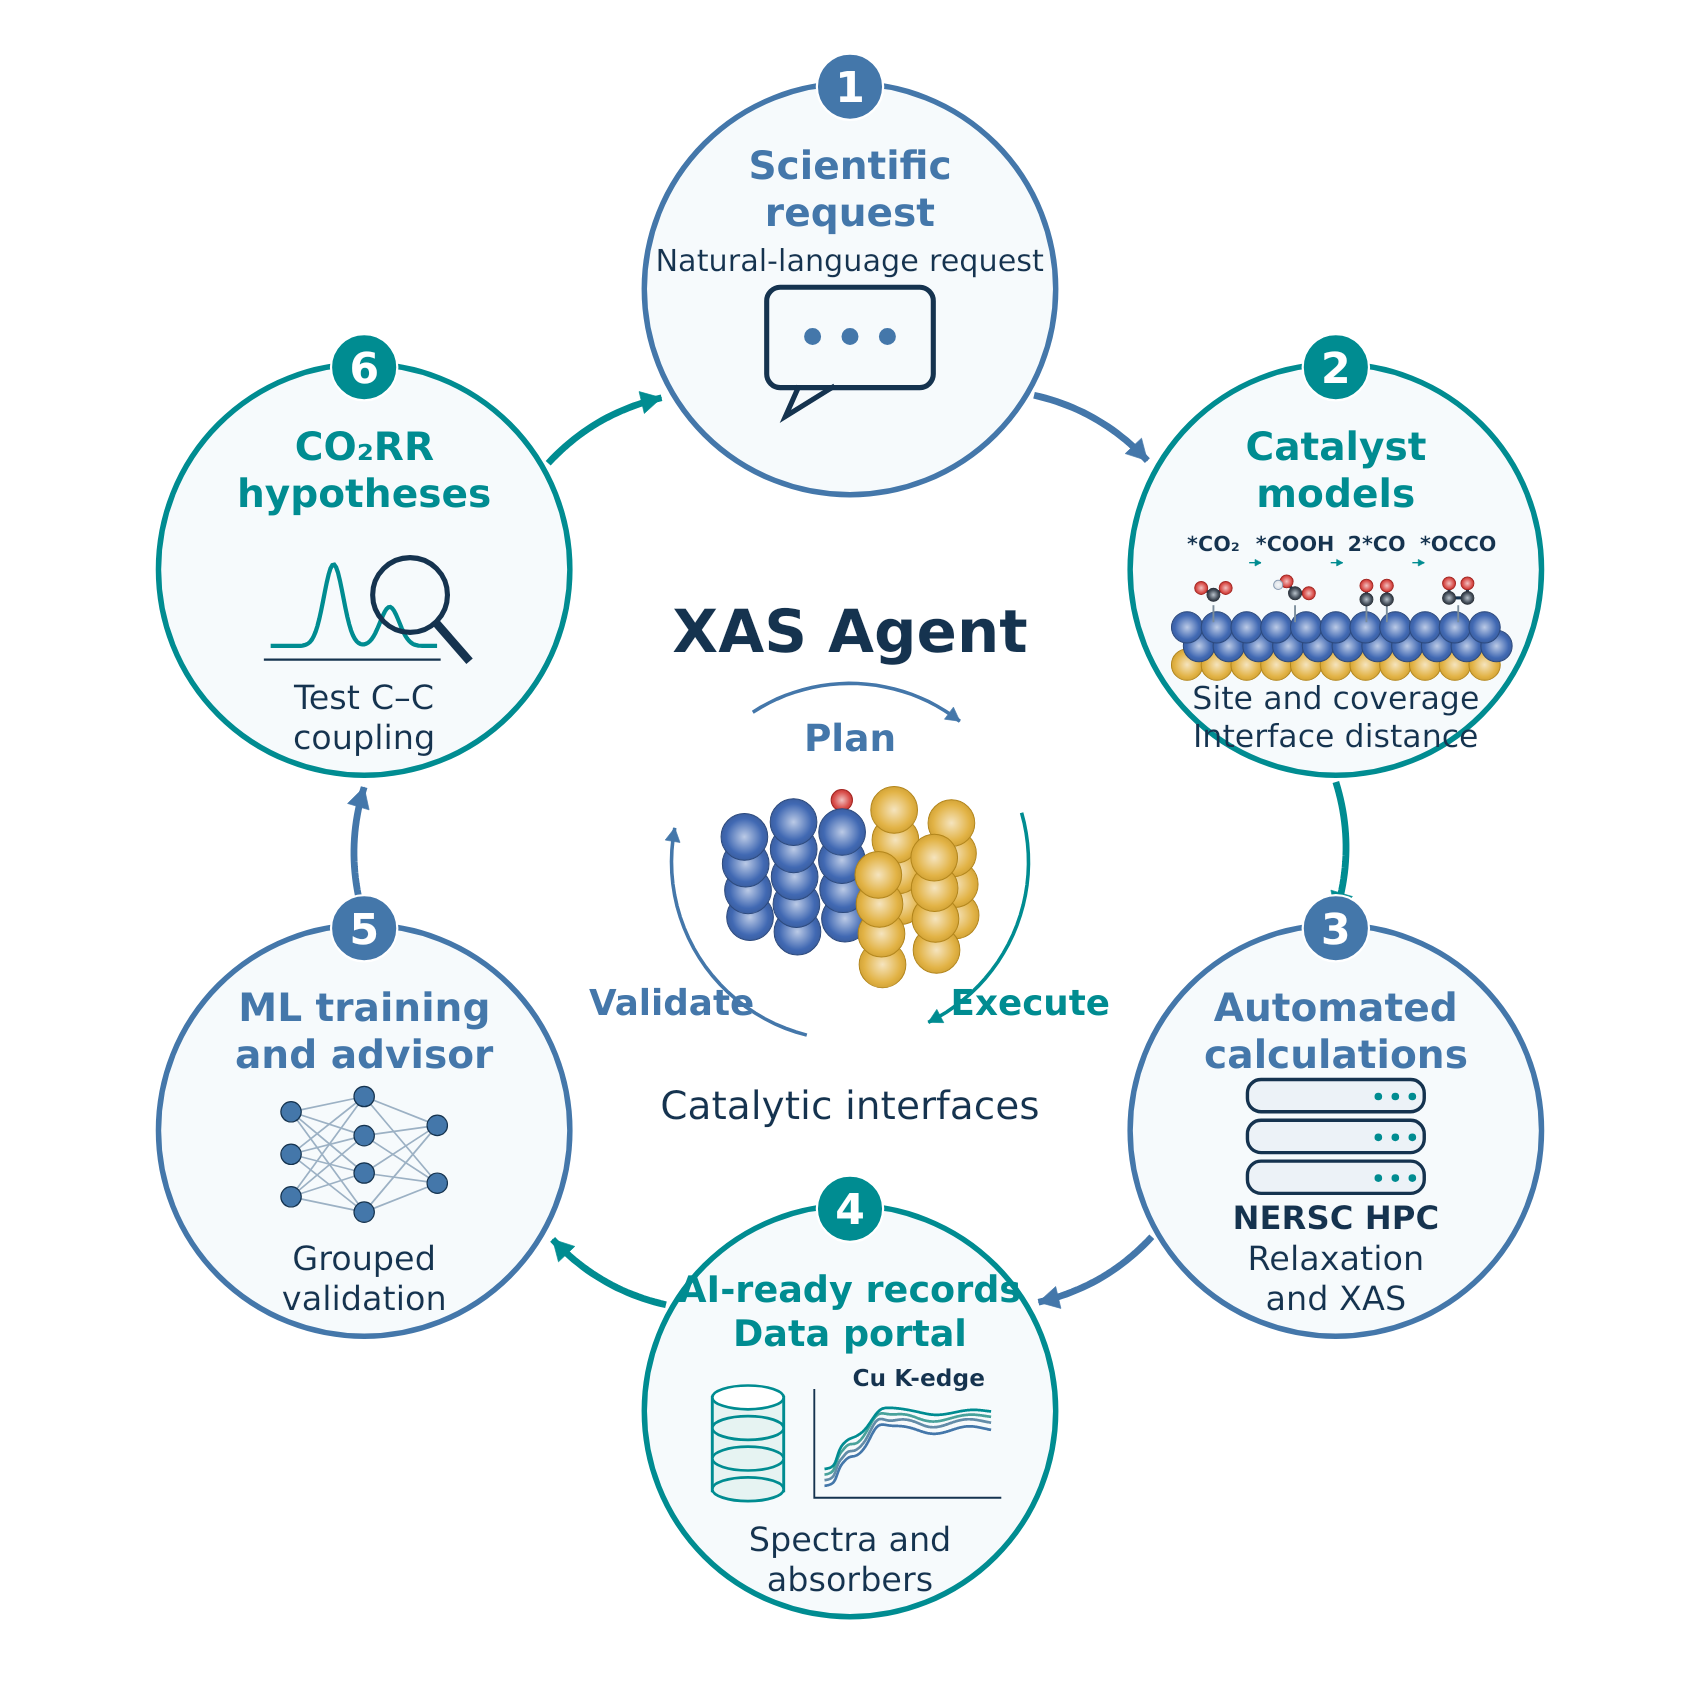
\includegraphics[width=.92\linewidth]{figures/Figure_1_framework.png}
\caption{Hypothesis-driven workflow for catalytic XAS. A scientific request specifies structural alternatives that are generated, relaxed, and evaluated by spectroscopy calculations. The calculation agent manages NERSC execution, and AI-ready records connect the outputs to model training and spectral interpretation. The return arrow represents refinement of the next calculation or hypothesis; it does not imply that a closed-loop catalytic discovery experiment has been completed.}
\label{fig:framework}
\end{figure}

The calculation agent manages remote calculations on the National Energy Research Scientific Computing Center (NERSC) Perlmutter supercomputer through authenticated interfaces.\cite{nersc} Within the specified allocation and numerical settings, it prepares and transfers inputs, submits and monitors scheduler jobs, and initiates XAS calculations after successful relaxation. Persistent calculation state allows monitoring and recovery to continue between user interactions. This coordination reduces manual file handling and permits routine calculations to advance with minimal intervention, while preserving the settings and structural identities needed for subsequent interpretation.

Relaxation is a scientific checkpoint because it determines which chemical state is actually probed. The spectrum is generated from the relaxed geometry, and the resulting record preserves the absorber ensemble and observed adsorbate identity. This prevents a requested OCCO starting model that separates into CO from being interpreted as evidence for a coupled state. The calculation stage and the dedicated analysis interface together cover model generation through predictive evaluation; automatic selection of the next catalytic experiment is a subsequent use of their outputs.

\subsection{Interfacial models and adsorbate configurations}
At a bimetallic interface, nominal composition alone cannot identify the environment responsible for a spectral change. CO bound to three Cu atoms and CO bound to one Cu and two Au atoms experience different local coordination even on the same parent surface. Conversely, an all-Cu binding motif can lie either near the boundary or on a Cu terrace. To distinguish these effects, each construction specifies the parent surface, the metal atoms defining the adsorption site, and the adsorbate's distance from the nearest interface (Fig.~\ref{fig:dataset}). Figure~\ref{fig:dataset}a shows the two structural ingredients separately: the Cu--Au substrate interface on the left and the adsorbate models on the right. The extended-surface illustration in Fig.~\ref{fig:dataset}c includes Cu and Au atop sites, Cu--Cu and boundary-spanning Cu--Au bridges, and CuCuCu, CuCuAu, and CuAuAu hollows. These configurations allow changes in local composition to be examined separately from changes in binding multiplicity or interface proximity.

\begin{figure}[!htbp]
\centering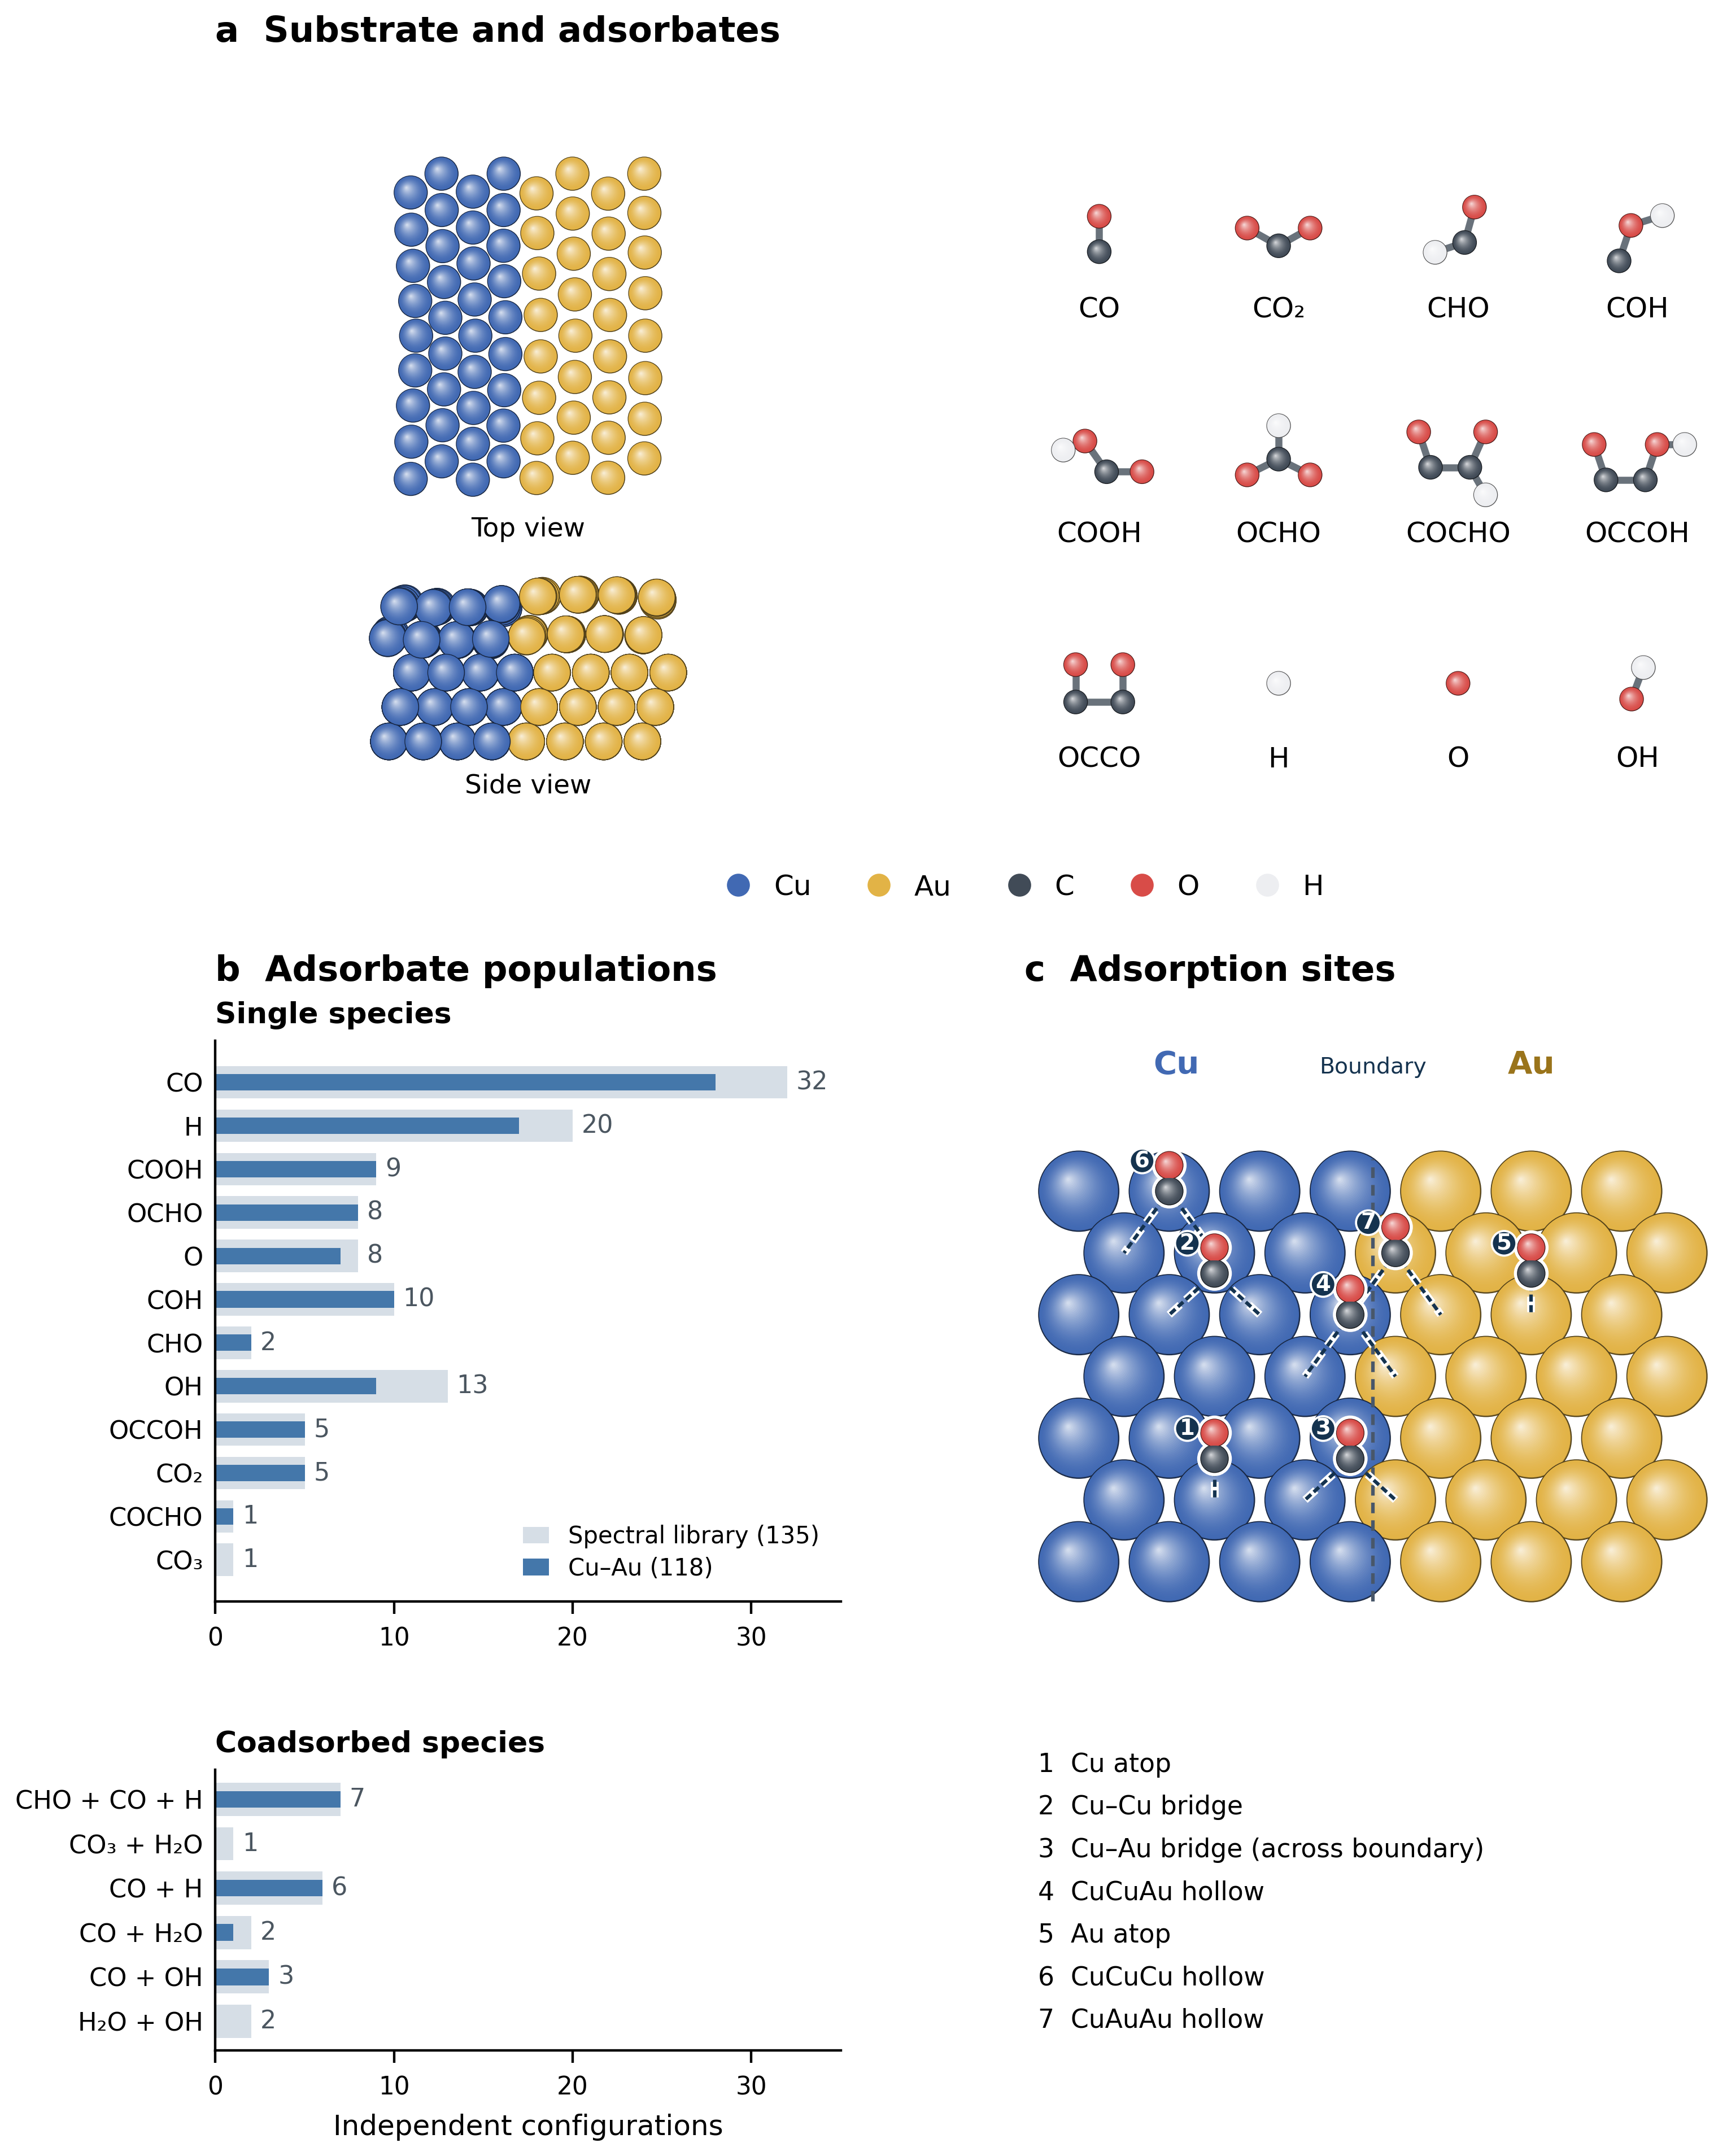
\includegraphics[width=\linewidth]{figures/Figure_2_dataset.png}
\caption{Substrate, adsorbate, and adsorption-site models. (a) Left: top and side views of the Cu--Au substrate from representative input coordinates. Right: schematic adsorbate structures, with one shared element legend. (b) Audited adsorbate-bearing spectral inventory: 118 Cu--Au and 17 Cu(100) adsorbate-bearing configurations. Broad gray bars count the full spectral inventory and narrow blue bars identify the Cu--Au subset; their difference is the Cu(100) contribution. A single-species configuration may contain several molecules. Clean references and configurations without compatible required-layer spectra or resolved geometry lineage are excluded. Cu(100) water/carbonate controls remain in the inventory. (c) Seven CO motifs on one schematic surface, including the boundary-spanning bridge and CuCuCu, CuCuAu and CuAuAu hollows.}
\label{fig:dataset}
\end{figure}

The Cu--Au construction space includes pure Cu(111) and Au(111) surfaces and lateral stripe ratios of 1:1, 2:1, 1:2, 3:1, and 1:3. Explicit row counts define the parent model, while adsorption positions distinguish boundary, neighboring-row, and terrace environments. These are the available structural controls; the completed cohort samples a subset of their combinations. At each location, coverage and spatial distribution determine how many metal environments are perturbed and whether adsorbates have nearby reaction partners. Molecular coverage is therefore retained together with its reference surface population. Carbon-equivalent coverage provides an additional comparison for OCCO and spectator CO, permitting equal carbon loading to be maintained when two CO molecules form one coupled intermediate.

Constructing these interfaces requires a common periodic length for metals with different lattice parameters. The agent searches integer repetitions of the two surface lattices and records the strain imposed on each domain. With the stored Cu and Au lattice constants, the automatic match combines nine Cu repeats with eight Au repeats, giving initial interface-parallel strains of approximately $+0.137\%$ and $-0.136\%$, respectively. This control matters chemically: lattice strain can change adsorption and carbon-coupling behavior,\cite{lei2022} while the associated changes in bond distances and electronic structure can also affect XAS. Recording the matching strain therefore helps distinguish changes associated with the chosen periodic model from those associated with an adsorbate or its proximity to the interface. A complementary construction mode searches for the smallest repeat pair satisfying a specified strain bound (5\% by default); the achieved strain and selected repeats are retained for each generated parent. These criteria concern the initial commensuration and do not constrain the local distortions that develop during relaxation.

Equal loading does not, however, imply equal chemical identity. Neighboring CO molecules remain an uncoupled state unless a C--C bond forms; separate CO and H likewise differ from bonded CHO. Molecular connectivity and metal contacts are checked after relaxation so that the spectral label describes the state actually calculated. Single-species and coadsorbed configurations are distinguished in Fig.~\ref{fig:dataset}b. Together, these controls make the dataset suitable for asking which spectral differences arise from chemistry and which arise from changes in the surrounding interface.

The current adsorbate-bearing Cu--Au inventory contains 101 single-species and 17 coadsorbed configurations. One water-containing configuration is retained in this inventory but excluded from the closed-label identity task. The latter contains 117 adsorbate-bearing configurations and one clean negative. Sampling is intentionally broad for CO, a small intermediate whose loading and proximity to a second CO molecule are central to proposed carbon-coupling pathways. Larger intermediates admit fewer nonoverlapping placements at the cell sizes considered, restricting both their accessible coverages and the number of distinct adsorption arrangements. This physical constraint contributes to unequal class support. Figure~\ref{fig:dataset}b counts exclusive identity sets, whereas classification support includes every configuration containing a species: the two CHO-only cases and seven CHO-containing mixtures, for example, provide nine CHO positives. These are configuration counts rather than counts of individual molecules or layer spectra.


\subsection{Scientific provenance and absorber averaging}
The records carry the information needed to decide whether two spectra constitute a controlled comparison. Adsorbate identity and molecular count specify the chemical alternatives; local coordination, interface distance, and coverage identify possible confounding changes. Absorber populations and calculation settings define how those structures contribute to the computed signal. Retaining these quantities together allows spectra to be regrouped for a new question without reconstructing their meaning from filenames. Coadsorption is treated as simultaneous species presence: CO+H contains two labels, while bonded CHO is a distinct molecular label. Structural descriptors define targets and support quality control; the classifiers reported here receive spectral features only.

A second hypothesis concerns observability: a real intermediate can be spectroscopically difficult to detect if most absorbers are far from it. Layer-resolved spectra separate this dilution question from changes in adsorbate identity. They permit surface and subsurface contributions to be examined for the same configuration. For layer means $\mu_l(E)$ representing $n_l$ Cu sites, a combined representation is formed as
\begin{equation}
\mu_D(E)=\frac{\sum_{l\in D}n_l\mu_l(E)}{\sum_{l\in D}n_l}.
\label{eq:average}
\end{equation}
Population weighting precedes spectral normalization. This preserves the physical meaning of a layer average and avoids assigning equal contributions to ensembles containing different numbers of absorbers. The same configuration is then evaluated through individual-layer and combined-layer representations, allowing depth sensitivity to be compared without changing the underlying sample population.


A clean five-layer Cu--Au parent was also relaxed with either the bottom three or bottom two metal layers fixed. Releasing the third layer changed the mean surface-to-subsurface spacing by only 0.0047~\AA{} in Cu and 0.0076~\AA{} in Au. The small spacing changes support the chosen constraint for the parent model, although the mean height of the surface Au atoms shifted by 0.138~\AA{}. This is a structural sensitivity check; corresponding spectral or adsorption-energy convergence is not inferred from these coordinates. The comparison and fixed-atom masks are documented in the Supporting Information.

The agent and analysis interface use a common training and inference implementation. It validates structural and reference compatibility, applies the specified grouped evaluation, and stores each model with its absorber populations, spectral units and preprocessing convention. Saved-model reloads test whether those definitions reproduce held-out inference. This integration preserves the physical meaning of the model input as the workflow advances from structure generation to prediction; the associated software validation is reported in the Supporting Information.

\section{Results and discussion}
\subsection{Cu K-edge reference benchmarks}
Cu, Cu$_2$O and CuO test the calculated Cu K-edge response across metallic, Cu(I) and Cu(II) environments (Fig.~\ref{fig:reference}). Fourteen material/method combinations provide complete numerical spectra, including Cu$_2$O calculated with both standard PBE and GW-type PAW datasets. The CuO PBE response is incomplete and is omitted from the spectral and similarity comparisons. The designation GW-PAW refers to the potential dataset; it does not establish a quasiparticle GW or Bethe--Salpeter treatment.

\begin{figure}[!htbp]\centering
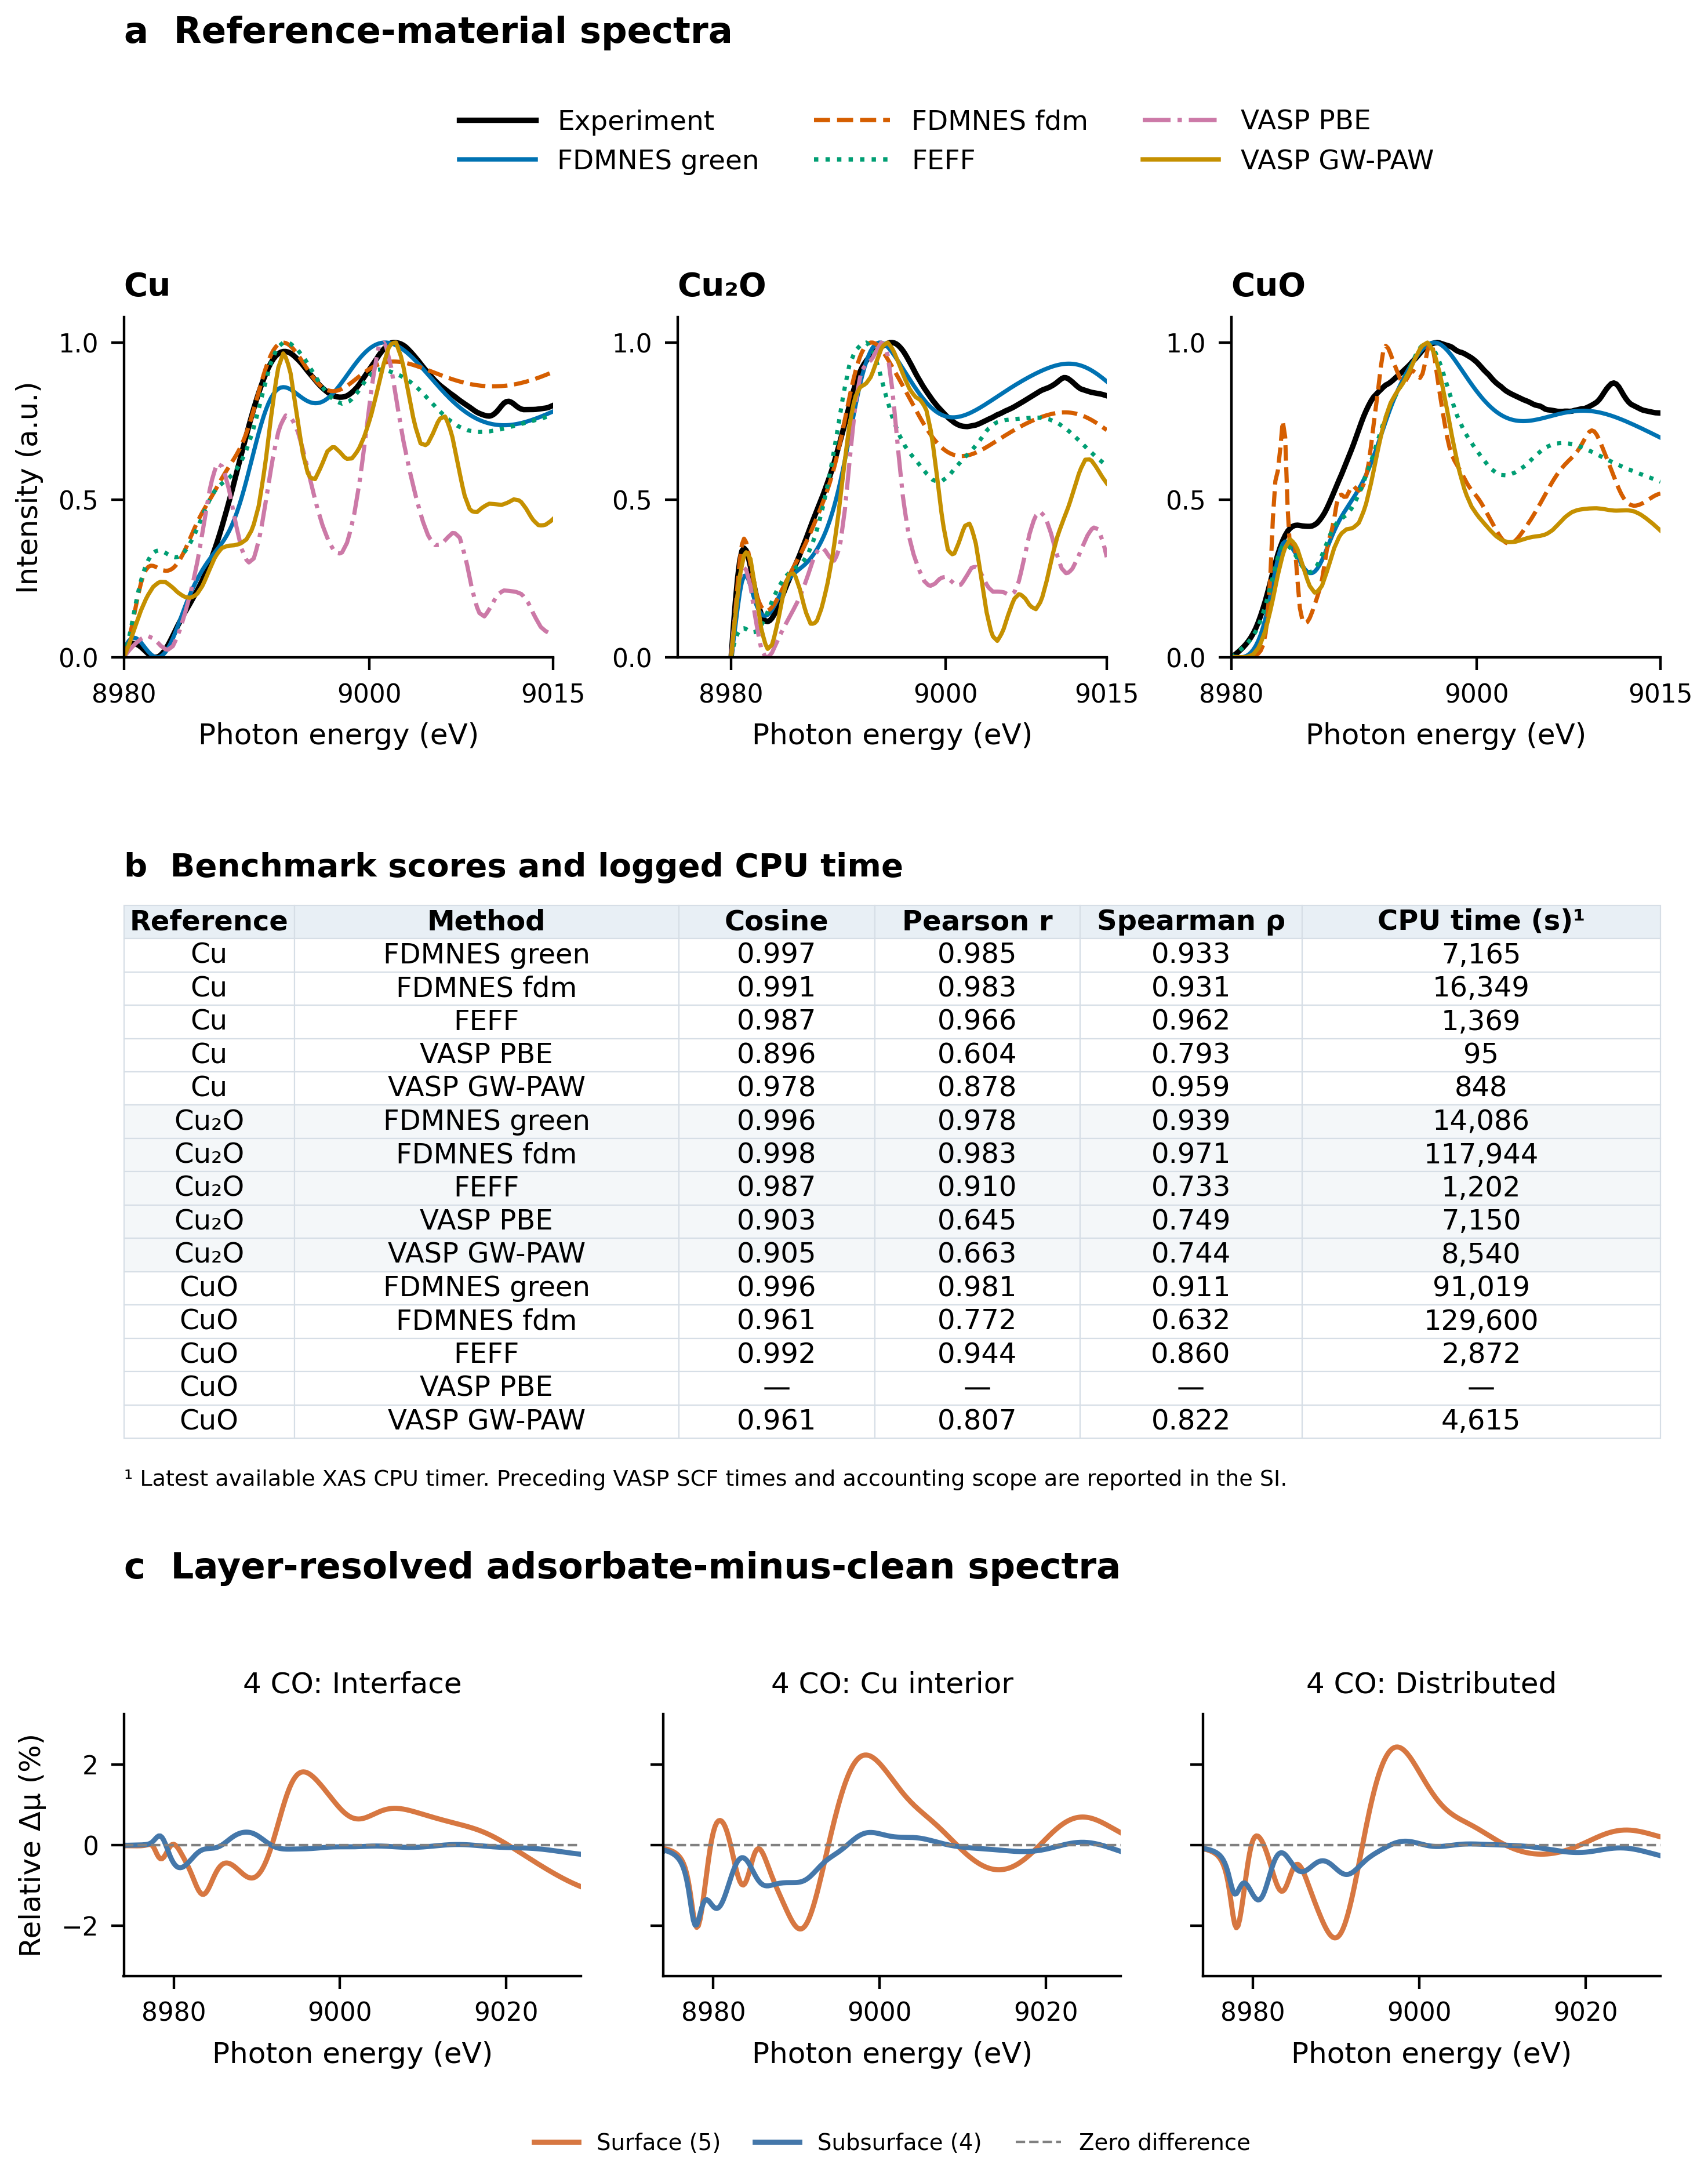
\includegraphics[width=\linewidth]{figures/Figure_3_spectroscopy.png}
\caption{Reference benchmarks and clean-referenced layer sensitivity. (a) Calculated spectra use first-feature alignment, the stated broadening and common intensity normalization. Cu$_2$O is displayed over 8975--9015 eV without extrapolating unsupported values; its FEFF curve retains Cu calibration. (b) Cosine, Pearson $r$ and Spearman $\rho$ use the plotted arrays on 8980--9015 eV. CPU values are the latest available XAS-stage counters in seconds; preceding VASP SCF times are reported separately in the Supporting Information. Native accounting scopes and resources differ. Missing CuO PBE scores remain blank. GW-PAW identifies the supplied PAW dataset, not a verified GW self-energy calculation. (c) Surface and subsurface adsorbed-minus-clean differences for three matched four-CO configurations, using one clean-derived intensity scale. Dashed gray denotes zero.}
\label{fig:reference}
\end{figure}

Reference spectra are compared after rigid energy alignment and a common intensity transformation. The small first Cu PBE peak is aligned at 8982 eV, rather than assigned to the later feature near 8993 eV. The Cu$_2$O comparison uses its first resolved peak, and CuO uses an early rising-edge inflection. VASP spectra retain the additional Gaussian width specified in the analysis notebook ($\sigma=1$ eV); the alignment changes neither this width nor the relative spacing of spectral features. All experimental and calculated curves are scaled using their own minimum and maximum over the same 8980--9015 eV interval. Similarities are calculated from these displayed arrays. A separate Cu-calibrated comparison in the Supporting Information applies each method's Cu offset to the oxides and therefore retains the test of transferable energy offsets.

Green-function FDMNES gives Pearson correlations of 0.985, 0.978 and 0.981 for Cu, Cu$_2$O and CuO. Finite differences slightly improve the Cu$_2$O correlation, whereas their CuO agreement is poorer. The metrics therefore support Green-function FDMNES as a practical route for the present configuration survey without establishing a universal accuracy ranking. Its multiple-scattering formulation provides an economical alternative to finite differences,\cite{joly2001,fdmnesmanual} but the available calculations do not constitute a controlled speed benchmark. In particular, VASP XAS follows a completed electronic-structure calculation at fixed ionic coordinates. Its saved charge density and wavefunctions provide a starting point for the chosen core-excited calculation, whose density treatment and Hamiltonian must remain consistent with the intended method. Figure~\ref{fig:reference}b reports one XAS CPU time per method; the preceding SCF times are provided in the Supporting Information. FEFF module timers are CPU times, and the author-verified CuO FDMNES finite-difference value is 129600 CPU s. Full timing provenance and resource limitations are given in the Supporting Information.

\subsection{Adsorbate identity and depth sensitivity}
The spectral library addresses two related questions: which adsorbates can be identified, and how much of that information survives averaging over deeper Cu layers? The fixed-depth benchmark in Fig.~\ref{fig:ml}a,c,d retains the original 87 independent configurations so that differences between depth representations are evaluated on identical structures. Each configuration contributes one spectrum for a given representation; its individual layer spectra never enter different folds as independent samples. Features and model settings are chosen inside the training partitions at each declared depth, without automatic selection of the sampling depth.

\begin{figure}[!htbp]\centering
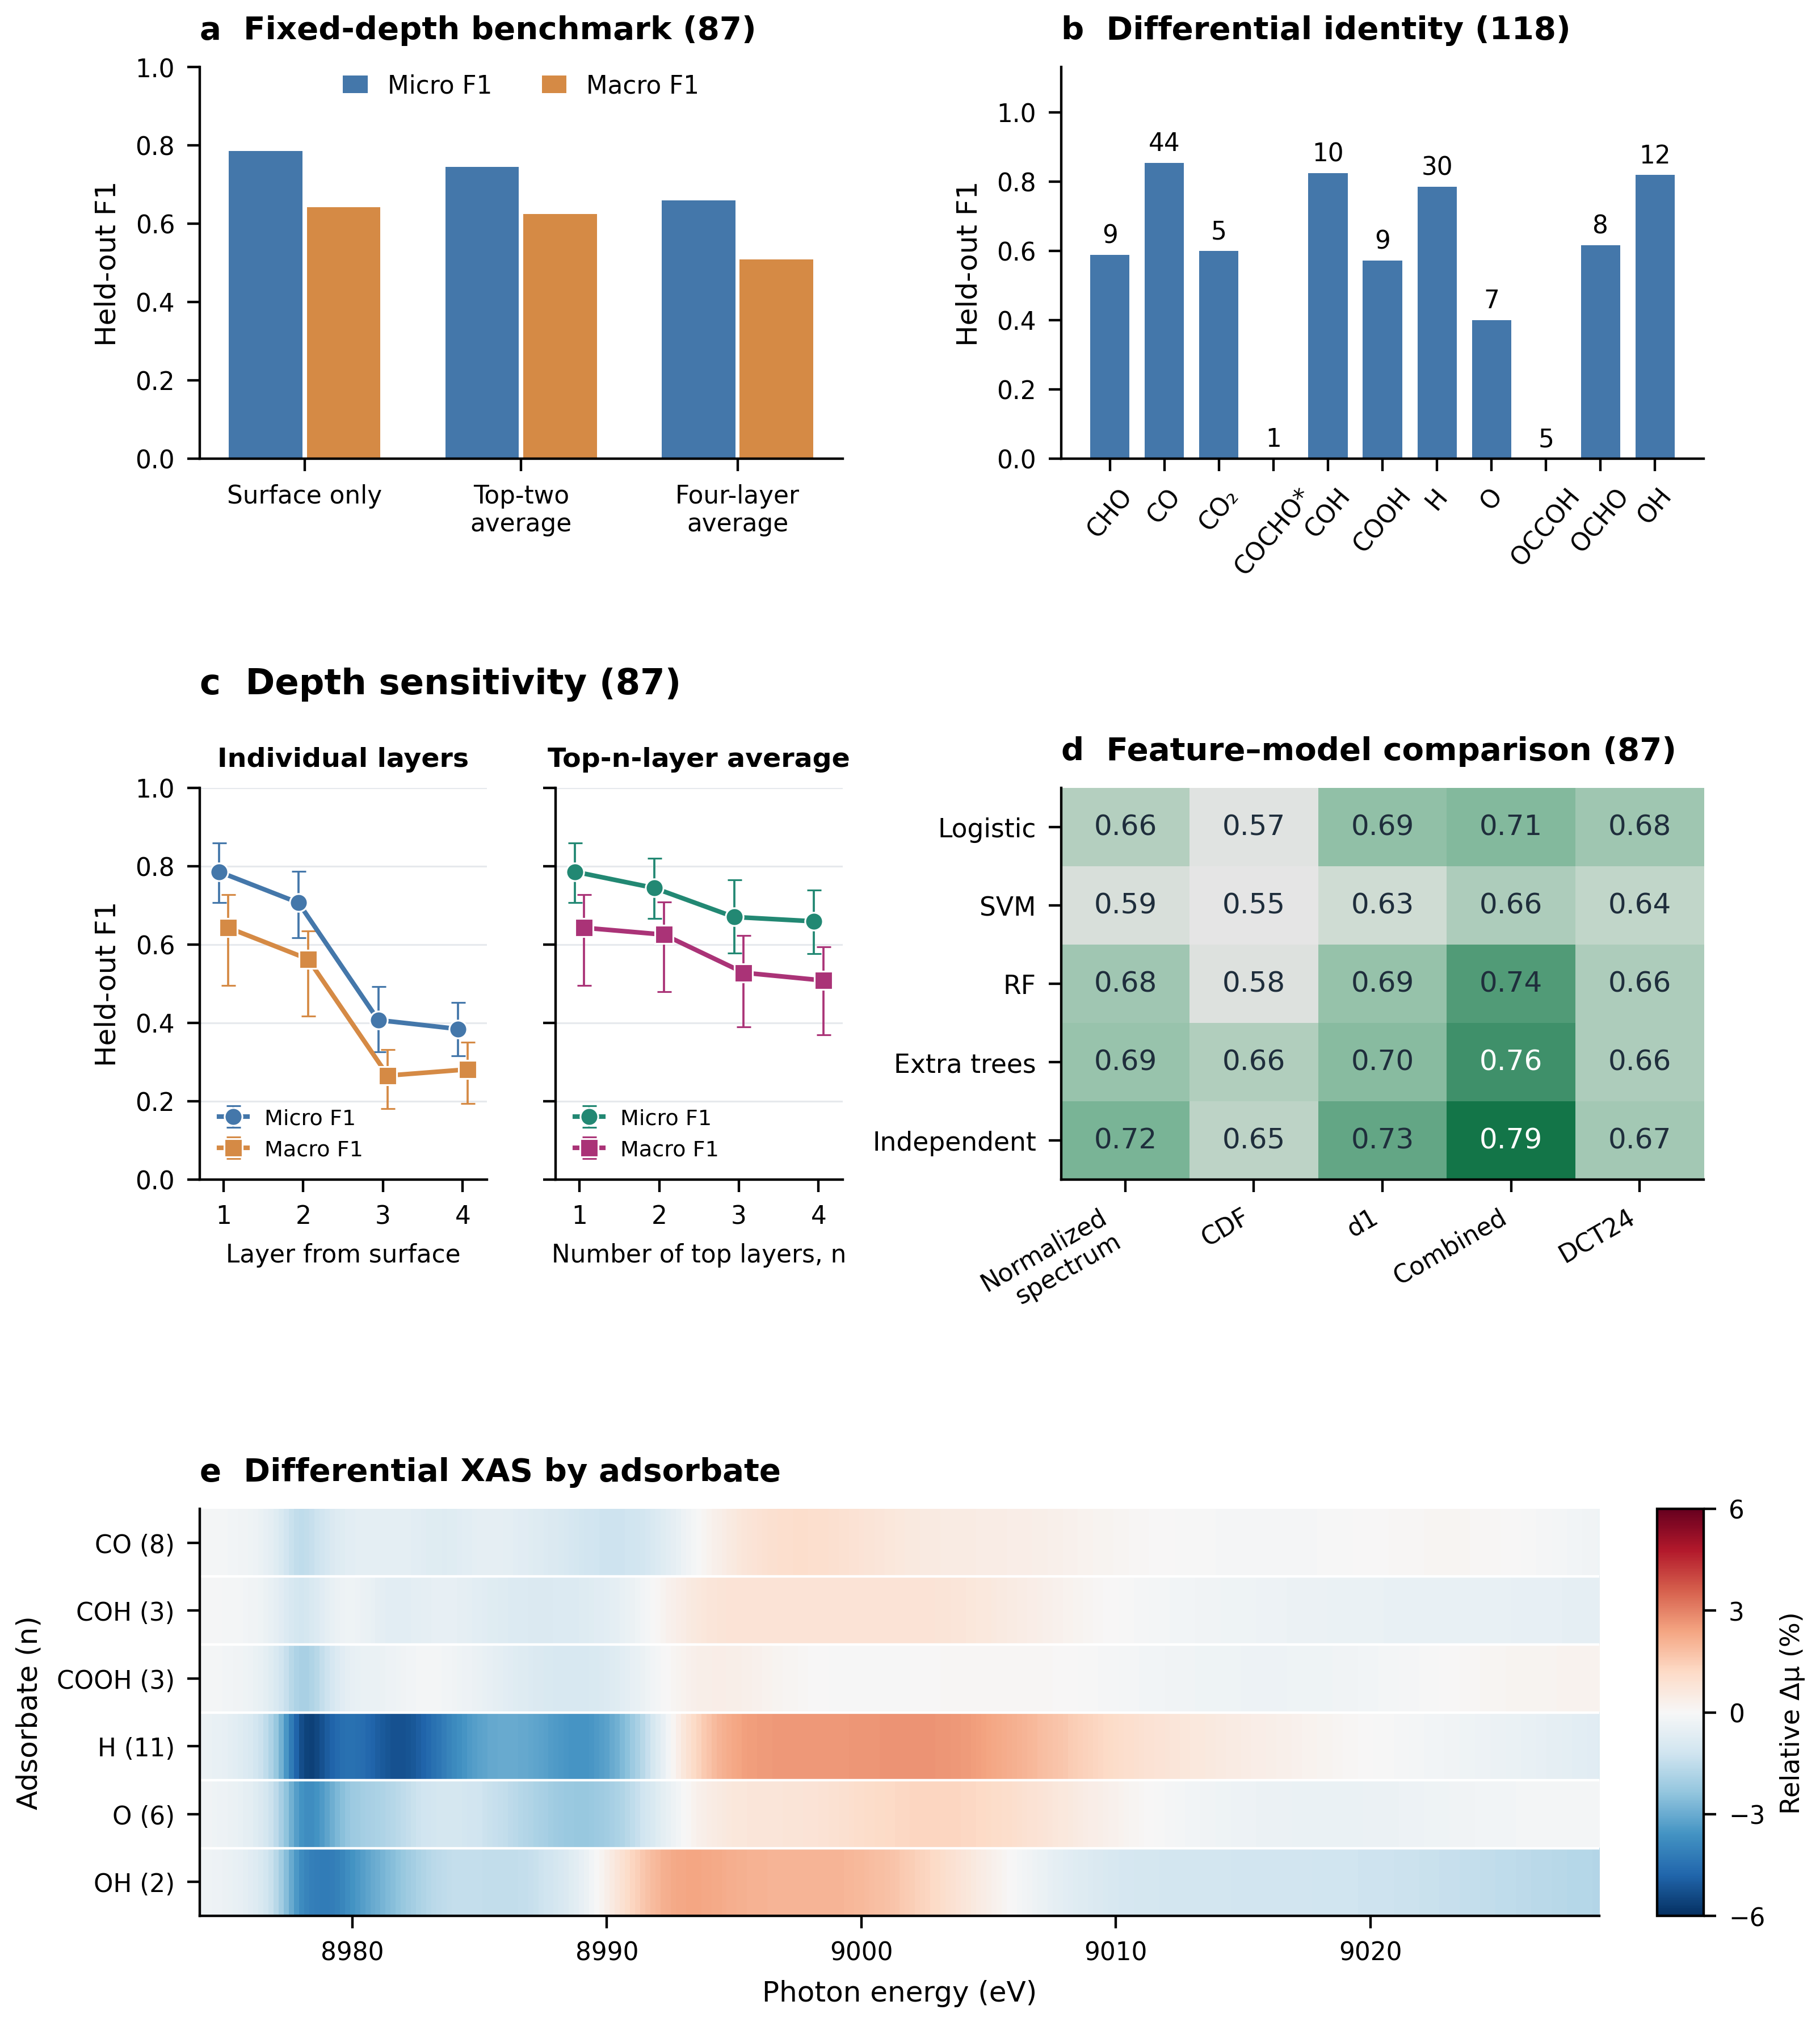
\includegraphics[width=\linewidth]{figures/Figure_4_ML.png}
\caption{Adsorbate identification, depth dependence and differential spectral response. (a) Fixed-depth micro/macro F1 on the 87-configuration depth benchmark. (b) Per-species held-out F1 for 118 Cu--Au configurations using signed differential top-two spectra. Numbers count independent positive configurations, including mixtures; asterisks denote fewer than five positives. Thus CHO has nine positives although only two configurations are CHO-only in Fig.~\ref{fig:dataset}b. (c) Individual-layer and population-weighted top-$n$ averages are shown in separate axes, each with micro and macro F1, on the 87-configuration benchmark. (d) Exploratory top-two feature/model comparison for the same 87 cases; green and gray indicate higher and lower micro F1. The depth and feature/model comparisons use the same 87 cases throughout. (e) Mean signed adsorbate-minus-clean spectra for the six single-species classes with matched initial substrate models. The 33 configurations are a subset of the 37 adsorbate-bearing cases with matching initial metal models and constraints; mixed configurations are excluded from this descriptive panel. All rows use the same physical reference and one symmetric color scale, expressed as a percentage of a shared clean-derived near-edge intensity scale. Numbers in parentheses are independent configuration counts. Between-species differences include coverage, site and substrate-relaxation effects as well as adsorbate chemistry.}
\label{fig:ml}
\end{figure}

For binary label indicators $y_{ik}$ and predictions $\hat y_{ik}$, the micro F1 aggregates true positives, false positives and false negatives across all configurations $i$ and labels $k$,
\begin{equation}
F_{1,\mathrm{micro}}=\frac{2\sum_k\mathrm{TP}_k}{2\sum_k\mathrm{TP}_k+\sum_k\mathrm{FP}_k+\sum_k\mathrm{FN}_k},
\qquad F_{1,\mathrm{macro}}=\frac{1}{K}\sum_{k=1}^{K}F_{1,k}.
\end{equation}
Exact-set accuracy additionally requires every predicted label to agree with the complete identity set of a configuration. These measures distinguish frequent-species recovery from performance across the full label set.

The surface layer carries the strongest identity signal, and adding deeper Cu layers progressively weakens it. On the fixed top-two representation, micro F1 is 0.744, compared with 0.659 for the average of all four available layers. The decline is consistent with a larger fraction of weakly perturbed absorbers entering the ensemble average. The individual-layer comparison shows that deeper layers also lose chemical discrimination on their own, rather than merely diluting a fixed surface signature. This depth analysis concerns the simulated slab and does not determine the absorber weighting of an experimental catalyst.

The expanded Cu--Au differential model gives micro/macro F1 of 0.719/0.550 across 118 configurations (Fig.~\ref{fig:ml}b). CO and COH are recovered more readily than the sparsely sampled coupled intermediates. These results use a compact grouped model comparison on the current cohort; they are distinct from the 87-configuration depth and feature comparisons. CHO has nine positive configurations but only two CHO-only cases, so its recovery also depends on distinguishing it from coadsorbates. For COCHO, the single positive leaves no positive training example when that configuration is held out. Its zero held-out F1 therefore cannot establish intrinsic spectral indistinguishability. The feature/model comparison in Fig.~\ref{fig:ml}d shows that inference also depends on representation and estimator; its highest score is exploratory rather than an independently validated optimum.

The normalized energy spectrum denotes intensity sampled on a fixed energy grid after the original minimum-subtracted unit-area transformation; the energy axis itself is unchanged. CDF is its cumulative integral, d1 its first energy derivative, and Combined includes the smoothed spectrum, integral and first/second derivatives. DCT24 retains the first 24 discrete-cosine coefficients, including the constant coefficient,\cite{ahmed1974} rather than 24 evenly spaced energies or frequencies. Definitions and equations are provided in the Supporting Information. The differential features introduced below preserve signed intensity and use signed cumulative differences rather than probability CDFs.

\subsection{Differential Cu K-edge response to adsorption}
The experimental target is an adsorption-associated change relative to a reference catalyst. We therefore use signed differential XAS on a shared relative scale, rather than requiring an absolute absorption cross-section per Cu atom. For reaction and reference spectra recorded and processed under compatible conditions,
\begin{equation}
d_i(E)=\frac{\mu_{\mathrm{ads},i}(E)-\mu_{\mathrm{ref},p(i)}(E)}{S_{p(i)}}.
\label{eq:delta}
\end{equation}
Here $S_p$ is a reference-derived intensity scale. A common multiplicative factor in both spectra and $S_p$ cancels; an absolute per-Cu calibration is therefore unnecessary for this observable. Already normalized experimental differences can be supplied directly when their energy, sign and normalization conventions are documented. This does not remove the need to assess relative energy registration, reference coverage and changes in the catalyst itself. Independently rescaling the two members can alter the adsorption contrast, while unit-normalizing a very weak difference can amplify noise. The intended experimental input thus retains the signed relative response and its uncertainty.

For the simulations, site spectra and convolution inputs establish comparable absorber averages before subtraction. Full explicit Cu-site lists contribute once per physical site; symmetry-reduced lists retain their verified multiplicities. This reconstruction is a simulation-side accounting step, not a requirement that experimental spectra be reported per Cu. Cu--Au uses layers 4+5, each with 36 Cu absorbers. A newly reconstructed clean Cu(100) reference uses layers 3+4, each with four Cu atoms, and verified symmetry weights. Its saved electronic spectra were convolved locally without a new electronic-structure calculation. The common simulated grid spans 8974--9029 eV, with $S_p$ defined by the difference between the clean-spectrum means over 9018--9025 and 8974--8977 eV. This short-window near-edge scale is a reproducible proxy, not a validated full experimental edge-jump normalization. Quantitative near-edge comparisons depend on normalization and the available energy range.\cite{weng2005,bugarin2024} Experiment and simulation require a compatible relative normalization convention before predictive transfer.

Thirty-seven adsorbate-bearing Cu--Au configurations share the clean model's initial metal coordinates and relaxation constraints. Of these, 33 contain a single species and define the class means in Fig.~\ref{fig:ml}e. A further 80 adsorbed Cu--Au cases have weaker initial-parent correspondence and are evaluated as same-substrate reference sensitivity. The clean negative is self-referenced. All comparisons include metal relaxation induced by adsorption, and coordinate equality alone does not prove independent ancestral lineage. The present dataset contains one reference family per substrate domain; it cannot establish transfer between independently prepared catalyst parents.

The clean-referenced means resolve changes in sign, amplitude and energy dependence for CO, COH, COOH, H, O and OH. Individual traces in the Supporting Information also show substantial within-species variation. Coverage, adsorption geometry, interface proximity and substrate relaxation contribute alongside molecular identity, so no class-mean extremum is assigned as a unique adsorbate fingerprint. These comparisons follow the motivation of adsorbate-sensitive difference XANES,\cite{ramaker2010,ramaker2014} while restricting chemical assignments to the simulated structures and absorber ensemble.

\subsection{Identity, CO loading and substrate dependence}
The current closed-label dataset contains 118 Cu--Au configurations, including one clean negative, and 12 Cu(100) configurations. Five Cu(100) water/carbonate controls and one Cu--Au CO/water case remain outside the eleven-label fitting task. Five configuration-held-out folds and grouped inner validation keep feature scaling, model selection and thresholds within the training data. Each representation uses the same configurations and folds. The compact comparison evaluates six predeclared feature/model combinations and is separate from the fixed-depth benchmark and training-size control.

\begin{figure}[!htbp]\centering
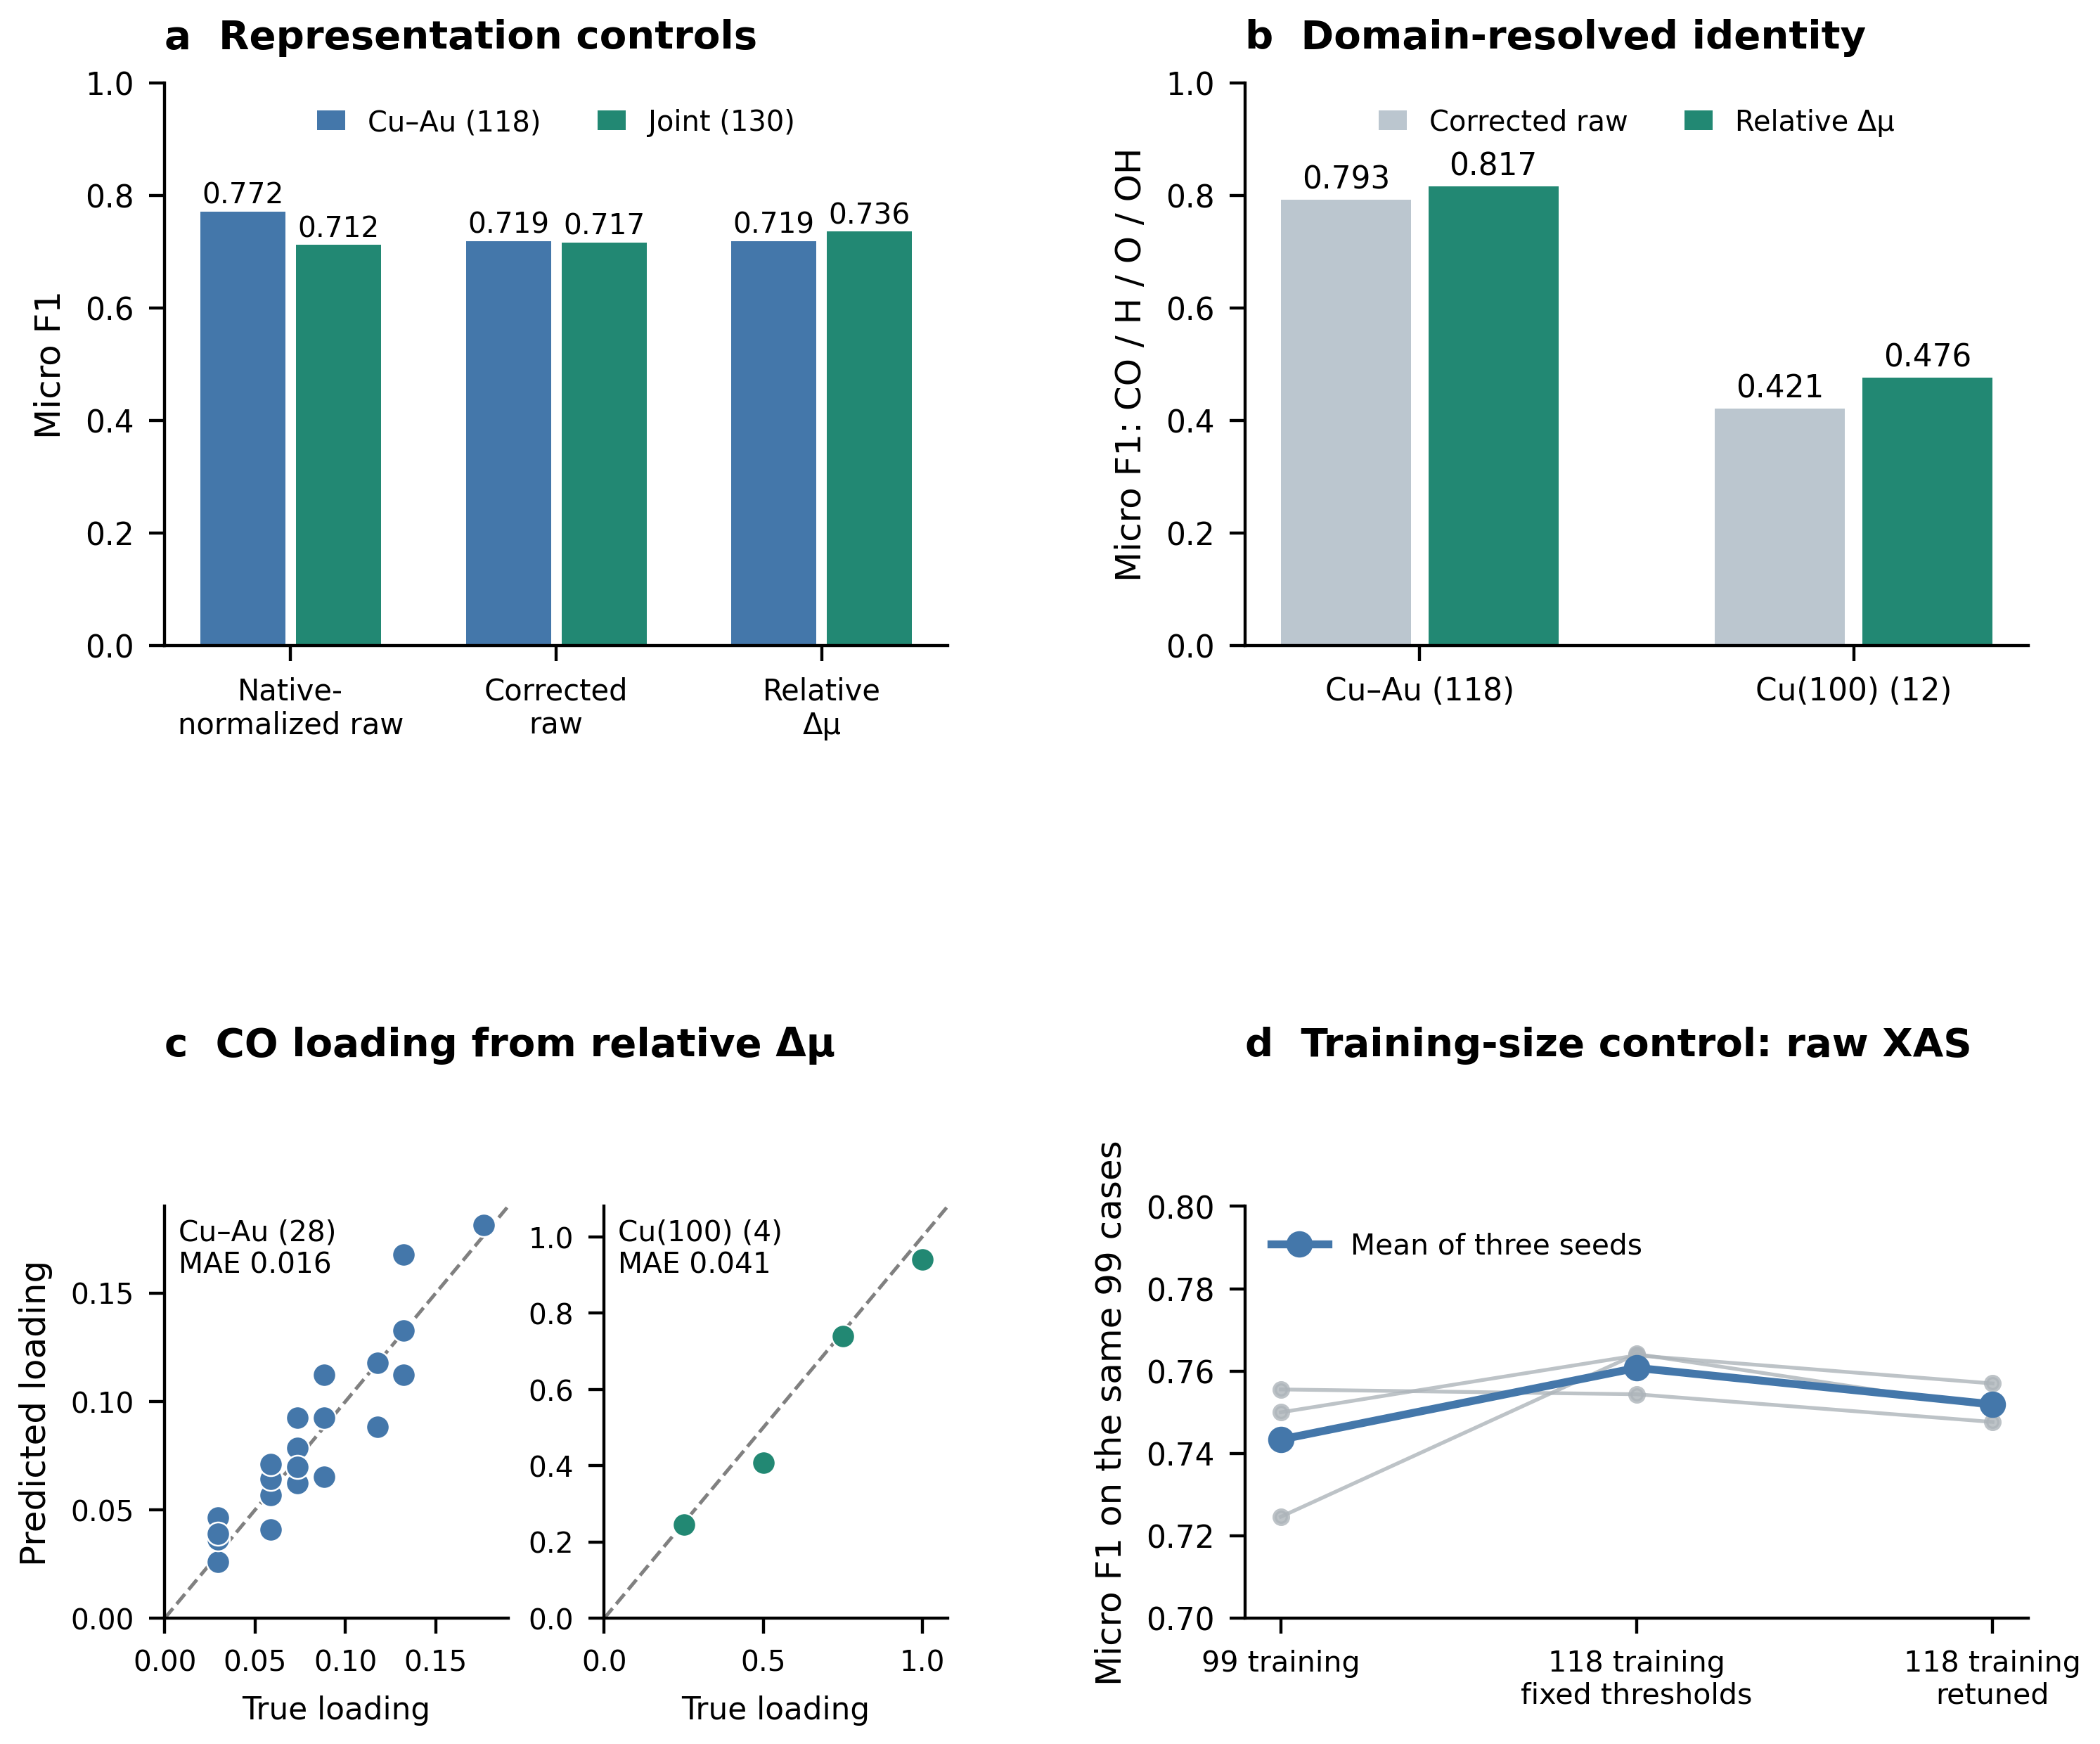
\includegraphics[width=\linewidth]{figures/Figure_5_reference_and_transfer.png}
\caption{Spectral representation, substrate dependence and training-set enlargement. (a) Micro F1 for 118 Cu--Au and 130 joint configurations using the same compact grouped protocol. Native-normalized raw uses the original convolution weighting followed by per-spectrum normalization; corrected raw and relative $\Delta\mu$ share reconstructed source weights and a clean-derived scale. Their comparison therefore does not isolate normalization from source weighting. (b) Joint-model scores on CO, H, O and OH are reported separately for Cu--Au and Cu(100). (c) Held-out CO-loading predictions from relative $\Delta\mu$, shown separately for 28 Cu--Au and four Cu(100) CO-only cases. Loading is CO per top-surface metal atom. Dashed lines indicate ideal predictions. (d) A separate normalized-raw, fixed-Combined training-size control evaluates the same 99 Cu--Au cases before and after enlargement to 118 training configurations. Thin gray lines show the three seeds; blue denotes their mean. Original training-derived thresholds are either transferred or retuned within training partitions. No automatic depth selection is used.}
\label{fig:newresults}
\end{figure}

On the Cu--Au cohort, corrected raw and differential spectra produce identical identity predictions, with micro F1 of 0.719 (Fig.~\ref{fig:newresults}a). A fixed clean spectrum is an affine translation and contributes no additional information in this comparison. The native-normalized control gives 0.772, but it changes both intensity normalization and source weighting. A corrected-and-normalized raw control is needed to separate these effects. With Cu(100) included, differential spectra give a pooled micro F1 of 0.736, compared with 0.717 for corrected raw. This conditional point difference neither establishes substrate invariance nor exceeds every Cu--Au-only control.

Domain-resolved results show why the pooled score is insufficient. For the four common labels CO, H, O and OH, the joint differential model gives micro F1 of 0.817 on Cu--Au and 0.476 on Cu(100) (Fig.~\ref{fig:newresults}b). Only twelve supported Cu(100) configurations are available, and the training folds contain other examples from that same substrate family. These tests assess configuration-held-out inference within sampled domains, rather than transfer to an unseen facet or parent. Mixtures remain more difficult than single species: the joint differential model recovers the complete identity set in only two of sixteen Cu--Au mixtures. Targeted coadsorption examples are therefore needed to separate the response of each component from changes in its chemical surroundings.

For CO loading, the target is $\theta_i=N_{\mathrm{CO},i}/N_{\mathrm{surface\ metal},i}$. Cu-normalized loading and CO/nm$^2$ are separately retained deterministic conversions; neither molecular count nor structural metadata enters the spectral predictor. For held-out predictions $\hat\theta_i$,
\begin{equation}
\mathrm{MAE}=\frac{1}{N}\sum_i|\hat\theta_i-\theta_i|,\qquad
R^2=1-\frac{\sum_i(\hat\theta_i-\theta_i)^2}{\sum_i(\theta_i-\bar\theta)^2}.
\end{equation}
Joint differential models give domain-specific MAE of 0.0159 on 28 Cu--Au and 0.0412 on four Cu(100) CO-only cases (Fig.~\ref{fig:newresults}c). The corresponding normalized-raw errors are 0.0109 and 0.0441. Pooled $R^2$ can be dominated by the between-domain loading range, and is not used as evidence of transfer. Applying CO-only models to CO-containing mixtures is an interference diagnostic rather than validation of general mixture-loading inference.

Local-coordination targets require additional structural diversity. Cu(100) contributes atop and bridge environments, but cannot substitute for the missing Au-rich hollow environments needed to distinguish Cu$_3$, Cu$_2$Au, CuAu$_2$ and Au$_3$. These hollow compositions and interface proximity are separate targets for CO and OCHO. Molecular site counts within a configuration do not increase the number of independent spectra. The available support therefore limits which site-specific catalytic hypotheses can presently be tested.

\subsection{Training-set size and chemical diversity}
To distinguish additional training data from a changing test set, the original 99 Cu--Au configurations retain their outer folds and are evaluated before and after adding 19 configurations. Both runs use the same top-two-layer normalized-raw Combined features, independent balanced ExtraTrees recipe and three fixed seeds. No depth or feature selector is rerun. The mean micro F1 increases from 0.7434 to 0.7519, while exact-set accuracy increases from 0.5993 to 0.6229 (Fig.~\ref{fig:newresults}d). Macro F1 changes little, from 0.5795 to 0.5812. Two seeds improve and one declines; each paired conditional micro-F1 interval crosses zero. Thus the data support a modest point gain, not a uniform or statistically established improvement. The full 118-case score evaluates a different query population and is not a paired learning-curve result.

Transferring the original training-derived thresholds gives a higher mean micro F1 of 0.7608 on the same 99 cases, indicating that threshold reselection can offset part of the point gain. This diagnostic does not justify selecting thresholds using outer-test scores. Likewise, adding three CO-only training configurations reduces MAE on the same 25 CO queries from 0.0140 to 0.0114, but its paired conditional interval still includes no improvement. These fixed-prediction intervals exclude model-refitting and parent-transfer uncertainty. The training-size experiment remains a raw-spectrum control; a fixed-recipe differential learning curve has not yet been evaluated.

The added structures do not uniformly expand chemical support. CO increases from 37 to 44 positive configurations and H from 25 to 30, whereas OCHO, COCHO and OCCOH remain at eight, one and five. Larger adsorbates occupy more surface area and permit fewer distinct nonoverlapping arrangements at a given cell size, contributing to this imbalance. Predictive gains consequently depend on whether additions fill missing chemical and structural environments, rather than only increasing the number of spectra. More independent examples of rare species, controlled mixtures and Au-rich binding motifs would address gaps left by further sampling of already common CO environments.

\subsection{Experimental observability and reference robustness}
Normalized experimental $\Delta\mu$ is the intended identity input. Its use does not require an absolute per-Cu intensity scale or an independently known surface fraction. The present models nevertheless require validation against experimental energy registration, normalization and noise. Synthetic stress tests in the Supporting Information examine shifts, gain errors, extra broadening, independent and shared-reference noise, and dilution. They diagnose sensitivity within simulated data rather than establish measured accuracy. A clean negative is falsely assigned COOH and OCCOH by the Cu--Au-only differential model, whereas the joint differential model returns the empty set for the same case. This limited control motivates validation of weak-signal detection and abstention before applying an identity model to small experimental differences.

Absolute coverage is more demanding than identity assignment. Unknown active surface fraction and detector or normalization gain can change differential amplitude without changing adsorbate chemistry. Coverage inferred from simulated surface-layer averages therefore requires a calibrated mapping to the measured absorber ensemble, or must be reported as a relative response or loading change. Subtracting a bulk background does not itself determine how many illuminated atoms belong to the reactive surface. Potential-induced oxidation, reconstruction, solvent and residual reference adsorbates can also contribute to $\Delta\mu$. Difference-XANES sensitivity motivates this approach,\cite{ramaker2010,ramaker2014} but compatible labeled measured references and independent parent surfaces remain necessary tests of its catalytic interpretation.

\subsection{Connectivity of water-containing coupling models}
A spectral test of C--C coupling requires an intact bonded intermediate and an uncoupled comparator at equal carbon loading on the same parent surface. The earlier three unfinished water-containing OCCO checkpoints had separated into 2CO, with C--C distances of approximately 3.28, 3.10 and 3.48~\AA. The expanded source audit also identifies the available OCCO/2H$_2$O top-layer spectral case as 2CO plus two water molecules. Its source geometry is retained as such and is excluded from the closed-label identity task because water is unsupported. Neither requested directory names nor incomplete relaxation trajectories establish a retained coupled intermediate or thermodynamic stability.

The absence of a retained coupled structure currently prevents attribution of a Cu K-edge difference specifically to C--C bond formation. A verified OCCO/2CO pair at fixed parent and carbon loading would provide the first such comparison. Repeating that comparison near the interface and on a Cu terrace would then test how Au proximity changes the coupling-associated signal. This distinction between requested and relaxed chemistry is essential to evaluating a catalytic pathway from simulated spectroscopy.

\section{Conclusions}
The framework connects catalytic hypotheses to validated structures, supercomputer XAS calculations and automated inference. The Cu--Au study resolves adsorbate information and its attenuation with absorber depth, while clean references expose adsorption-associated spectral changes. A shared relative differential scale provides a route toward normalized experimental inputs without requiring absolute per-Cu absorption. The expanded data yield modest but inconclusive gains in controlled identity and CO-loading tests. Rare chemical states, coadsorbate interactions and substrate dependence remain the principal limits. Differential subtraction alone does not resolve them: with a fixed reference, it adds no information beyond the corresponding raw signal. Experimental validation must distinguish identity inference from absolute coverage calibration and test independent catalyst/reference families. Preserving the link between the requested hypothesis, the relaxed chemical state and its spectral response makes those next comparisons both interpretable and reproducible.

\section*{Data and code availability}
Versioned source packages, corrected records, paired arrays, fold assignments, saved models, held-out predictions, numerical reference benchmarks and figure-generation code are available through the study repository at \url{https://github.com/HailiJia/CO2RR_XAS_agent}. The preserved benchmark and updated analyses are identified separately in the accompanying data.
\section*{Acknowledgements}
This work used resources of the Center for Nanoscale Materials, a U.S. Department of Energy Office of Science User Facility at Argonne National Laboratory.
\begingroup\small\setlength{\parskip}{0pt}
\begin{thebibliography}{99}
\bibitem{ni2024} W. Ni, H. Chen, N. Tang \textit{et al.}, High-purity ethylene production via indirect carbon dioxide electrochemical reduction, \textit{Nat. Commun.}, 2024, \textbf{15}, 6078, DOI: \href{https://doi.org/10.1038/s41467-024-50522-7}{10.1038/s41467-024-50522-7}.
\bibitem{francis2018} S. A. Francis, J. M. Velazquez, I. M. Ferrer, D. A. Torelli, D. Guevarra, M. T. McDowell, K. Sun, X. Zhou, F. H. Saadi, J. John, M. H. Richter, F. P. Hyler, K. M. Papadantonakis, B. S. Brunschwig and N. S. Lewis, Reduction of aqueous CO\textsubscript{2} to 1-propanol at MoS\textsubscript{2} electrodes, \textit{Chem. Mater.}, 2018, \textbf{30}, 4902--4908, DOI: \href{https://doi.org/10.1021/acs.chemmater.7b04428}{10.1021/acs.chemmater.7b04428}.
\bibitem{zhan2024} C. Zhan, F. Dattila, C. Rettenmaier, A. Herzog, M. Herran, T. Wagner, F. Scholten, A. Bergmann, N. L\'opez and B. Roldan Cuenya, Key intermediates and Cu active sites for CO\textsubscript{2} electroreduction to ethylene and ethanol, \textit{Nat. Energy}, 2024, \textbf{9}, 1485--1496, DOI: \href{https://doi.org/10.1038/s41560-024-01633-4}{10.1038/s41560-024-01633-4}.
\bibitem{montoya2015} J. H. Montoya, C. Shi, K. Chan and J. K. N\o rskov, Theoretical insights into a CO dimerization mechanism in CO\textsubscript{2} electroreduction, \textit{J. Phys. Chem. Lett.}, 2015, \textbf{6}, 2032--2037, DOI: \href{https://doi.org/10.1021/acs.jpclett.5b00722}{10.1021/acs.jpclett.5b00722}.
\bibitem{operando2021} J. Timoshenko and B. Roldan Cuenya, In situ/operando electrocatalyst characterization by X-ray absorption spectroscopy, \textit{Chem. Rev.}, 2021, \textbf{121}, 882--961, DOI: \href{https://doi.org/10.1021/acs.chemrev.0c00396}{10.1021/acs.chemrev.0c00396}.
\bibitem{lin2020} S.-C. Lin, C.-C. Chang, S.-Y. Chiu, H.-T. Pai, T.-Y. Liao, C.-S. Hsu, W.-H. Chiang, M.-K. Tsai and H. M. Chen, Operando time-resolved X-ray absorption spectroscopy reveals the chemical nature enabling highly selective CO\textsubscript{2} reduction, \textit{Nat. Commun.}, 2020, \textbf{11}, 3525, DOI: \href{https://doi.org/10.1038/s41467-020-17231-3}{10.1038/s41467-020-17231-3}.
\bibitem{morales2018} C. G. Morales-Guio, E. R. Cave, S. A. Nitopi, J. T. Feaster, L. Wang, K. P. Kuhl, A. Jackson, N. C. Johnson, D. N. Abram, T. Hatsukade, C. Hahn and T. F. Jaramillo, Improved CO\textsubscript{2} reduction activity towards C\textsubscript{2+} alcohols on a tandem gold on copper electrocatalyst, \textit{Nat. Catal.}, 2018, \textbf{1}, 764--771, DOI: \href{https://doi.org/10.1038/s41929-018-0139-9}{10.1038/s41929-018-0139-9}.
\bibitem{rehr2010} J. J. Rehr, J. J. Kas, F. D. Vila, M. P. Prange and K. Jorissen, Parameter-free calculations of X-ray spectra with FEFF9, \textit{Phys. Chem. Chem. Phys.}, 2010, \textbf{12}, 5503--5513, DOI: \href{https://doi.org/10.1039/B926434E}{10.1039/B926434E}.
\bibitem{joly2001} Y. Joly, X-ray absorption near-edge structure calculations beyond the muffin-tin approximation, \textit{Phys. Rev. B}, 2001, \textbf{63}, 125120, DOI: \href{https://doi.org/10.1103/PhysRevB.63.125120}{10.1103/PhysRevB.63.125120}.
\bibitem{vasp1996} G. Kresse and J. Furthm\"uller, Efficient iterative schemes for ab initio total-energy calculations using a plane-wave basis set, \textit{Phys. Rev. B}, 1996, \textbf{54}, 11169--11186, DOI: \href{https://doi.org/10.1103/PhysRevB.54.11169}{10.1103/PhysRevB.54.11169}.
\bibitem{vaspxas} VASP Wiki, Supercell core-hole calculations, \url{https://vasp.at/wiki/index.php/SCH_calculations}, accessed 21 October 2026.
\bibitem{ocean2011} J. Vinson, J. J. Rehr, J. J. Kas and E. L. Shirley, Bethe--Salpeter equation calculations of core excitation spectra, \textit{Phys. Rev. B}, 2011, \textbf{83}, 115106, DOI: \href{https://doi.org/10.1103/PhysRevB.83.115106}{10.1103/PhysRevB.83.115106}.
\bibitem{timoshenko2018} J. Timoshenko, A. Anspoks, A. Cintins, A. Kuzmin, J. Purans and A. I. Frenkel, Neural network approach for characterizing structural transformations by X-ray absorption fine structure spectroscopy, \textit{Phys. Rev. Lett.}, 2018, \textbf{120}, 225502, DOI: \href{https://doi.org/10.1103/PhysRevLett.120.225502}{10.1103/PhysRevLett.120.225502}.
\bibitem{marcella2020} N. Marcella, Y. Liu, J. Timoshenko, E. Guan, M. Luneau, T. Shirman, A. M. Plonka, J. E. S. van der Hoeven, J. Aizenberg, C. M. Friend and A. I. Frenkel, Neural network assisted analysis of bimetallic nanocatalysts using X-ray absorption near edge structure spectroscopy, \textit{Phys. Chem. Chem. Phys.}, 2020, \textbf{22}, 18902--18910, DOI: \href{https://doi.org/10.1039/D0CP02098B}{10.1039/D0CP02098B}.
\bibitem{torrisi2020} S. B. Torrisi, M. R. Carbone, B. A. Rohr, J. H. Montoya, Y. Ha, J. Yano, S. K. Suram and L. Hung, Random forest machine learning models for interpretable X-ray absorption near-edge structure spectrum-property relationships, \textit{npj Comput. Mater.}, 2020, \textbf{6}, 109, DOI: \href{https://doi.org/10.1038/s41524-020-00376-6}{10.1038/s41524-020-00376-6}.
\bibitem{david2023} T. David, N. K. Nik Aznan, K. Garside and T. J. Penfold, Towards the automated extraction of structural information from X-ray absorption spectra, \textit{Digital Discovery}, 2023, \textbf{2}, 1461--1470, DOI: \href{https://doi.org/10.1039/D3DD00101F}{10.1039/D3DD00101F}.
\bibitem{chen2024} Y. Chen, C. Chen, I. Hwang, M. J. Davis, W. Yang, C. Sun, G.-H. Lee, D. McReynolds, D. Allan, J. Marulanda Arias, S. P. Ong and M. K. Y. Chan, Robust machine learning inference from X-ray absorption near edge spectra through featurization, \textit{Chem. Mater.}, 2024, \textbf{36}, 2304--2313, DOI: \href{https://doi.org/10.1021/acs.chemmater.3c02584}{10.1021/acs.chemmater.3c02584}.
\bibitem{jia2026} H. Jia, Y. Chen, G.-H. Lee, J. Smith, M. Chi, W. Yang and M. K. Y. Chan, Revealing local structures through machine-learning-fused multimodal spectroscopy, \textit{ACS Nano}, 2026, \textbf{20}, 4228--4240, DOI: \href{https://doi.org/10.1021/acsnano.5c16942}{10.1021/acsnano.5c16942}.
\bibitem{bran2024} A. M. Bran, S. Cox, O. Schilter, C. Baldassari, A. D. White and P. Schwaller, Augmenting large language models with chemistry tools, \textit{Nat. Mach. Intell.}, 2024, \textbf{6}, 525--535, DOI: \href{https://doi.org/10.1038/s42256-024-00832-8}{10.1038/s42256-024-00832-8}.
\bibitem{canty2023} R. B. Canty, B. A. Koscher, M. A. McDonald and K. F. Jensen, Integrating autonomy into automated research platforms, \textit{Digital Discovery}, 2023, \textbf{2}, 1259--1268, DOI: \href{https://doi.org/10.1039/D3DD00135K}{10.1039/D3DD00135K}.
\bibitem{vriza2026} A. Vriza \textit{et al.}, Multi-agentic AI framework for end-to-end atomistic simulations, \textit{Digital Discovery}, 2026, \textbf{5}, 440--452, DOI: \href{https://doi.org/10.1039/D5DD00435G}{10.1039/D5DD00435G}.
\bibitem{nersc} NERSC, The Superfacility API, \url{https://docs.nersc.gov/services/sfapi/}, accessed 21 October 2026.
\bibitem{fdmnesmanual} Y. Joly, \textit{FDMNES User's Guide}, November 2022, \url{https://data-analysis.synchrotron-soleil.fr/tmp/software/fdmnes/fdmnes_Linux/Doc/Manual_Eng.pdf}, accessed 21 October 2026.
\bibitem{ahmed1974} N. Ahmed, T. Natarajan and K. R. Rao, Discrete cosine transform, \textit{IEEE Trans. Comput.}, 1974, \textbf{C-23}, 90--93, DOI: \href{https://doi.org/10.1109/T-C.1974.223784}{10.1109/T-C.1974.223784}.
\bibitem{geurts2006} P. Geurts, D. Ernst and L. Wehenkel, Extremely randomized trees, \textit{Mach. Learn.}, 2006, \textbf{63}, 3--42, DOI: \href{https://doi.org/10.1007/s10994-006-6226-1}{10.1007/s10994-006-6226-1}.
\bibitem{montoya2013} J. H. Montoya, A. A. Peterson and J. K. N\o rskov, Insights into C--C coupling in CO\textsubscript{2} electroreduction on copper electrodes, \textit{ChemCatChem}, 2013, \textbf{5}, 737--742, DOI: \href{https://doi.org/10.1002/cctc.201200564}{10.1002/cctc.201200564}.
\bibitem{ramaker2010} D. E. Ramaker and D. C. Koningsberger, The atomic AXAFS and Delta mu XANES techniques as applied to heterogeneous catalysis and electrocatalysis, \textit{Phys. Chem. Chem. Phys.}, 2010, \textbf{12}, 5514--5534, DOI: \href{https://doi.org/10.1039/B927120C}{10.1039/B927120C}.
\bibitem{ramaker2014} D. E. Ramaker, A. Korovina, V. Croze, J. Melke and C. Roth, Following ORR intermediates adsorbed on a Pt cathode catalyst during break-in of a PEM fuel cell by in operando X-ray absorption spectroscopy, \textit{Phys. Chem. Chem. Phys.}, 2014, \textbf{16}, 13645--13653, DOI: \href{https://doi.org/10.1039/C4CP00192C}{10.1039/C4CP00192C}.
\bibitem{lei2022} Q. Lei, L. Huang, J. Yin \textit{et al.}, Structural evolution and strain generation of derived-Cu catalysts during CO\textsubscript{2} electroreduction, \textit{Nat. Commun.}, 2022, \textbf{13}, 4857, DOI: \href{https://doi.org/10.1038/s41467-022-32601-9}{10.1038/s41467-022-32601-9}.
\bibitem{weng2005} T.-C. Weng, G. S. Waldo and J. E. Penner-Hahn, A method for normalization of X-ray absorption spectra, \textit{J. Synchrotron Rad.}, 2005, \textbf{12}, 506--510, DOI: \href{https://doi.org/10.1107/S0909049504034193}{10.1107/S0909049504034193}.
\bibitem{bugarin2024} L. Bugarin, H. A. Suarez Orduz and P. Glatzel, Area normalization of HERFD-XANES spectra, \textit{J. Synchrotron Rad.}, 2024, \textbf{31}, 1118--1125, DOI: \href{https://doi.org/10.1107/S1600577524005307}{10.1107/S1600577524005307}.
\end{thebibliography}

\endgroup
\end{document}
